\documentclass[deligne.tex]{subfiles}

\begin{document}
\subsection*{Sasha's exposé}
Sasha gave (12/5/19) a lecture outlining how to glue perverse
sheaves based on his article, which he says was written in a language
somewhat better suited to $\mathcal D$-modules, so he gave an exposé
tailored to perverse sheaves. This section is an attempt to write down the
contents of his exposé.

\begin{equation*}\begin{tikzcd}
	Y\arrow[r,hook,"i"]&X\arrow[d,"f"]&U\arrow[l,hook',"j"'] \\
	&\A^1
\end{tikzcd}\end{equation*}
The theorem is that the functor
\begin{equation*}\begin{tikzcd}[column sep=0pt]
	\mathcal F\longmapsto(&\mathcal F_Y\arrow[d,equals],
	&\mathcal F_U\arrow[d,equals],&\text{gluing datum}) \\
	&\Psi^{\mathrm{un}}_f\mathcal F
	&\mathcal F_U
	&\mathcal F_Y\rightleftarrows \Psi^{\mathrm{un}}_f\mathcal F_U
\end{tikzcd}\end{equation*}
is an equivalence of categories between perverse sheaves on $X$ and
perverse sheaves on $U$ and $Y$ with a gluing datum which consists of 
morphisms arising (up to a twist) from composing arrows coming from
\begin{equation*}
	\Psi^{\mathrm{un}}\xra{\operatorname{can}}
	\Phi^{\mathrm{un}}\xra{\operatorname{var}}
	\Psi^{\mathrm{un}}(-1)
\end{equation*}
where $\operatorname{var}$ denotes variation. Choosing a generator for
$\ZZ_\ell(1)$, the composition of these arrows gives $1-t$ 
(c.f. \cite[Exp. XIII 1.4]{SGA7}).
Now for the definition of the unipotent nearby and vanishing cycles.
\begin{equation*}\begin{tikzcd}[row sep=tiny]
	&&\overline U\arrow[dd,"\pi"]\arrow[dr] \\
	&&&\tilde U\arrow[dl,"\tilde\pi"] \\
	Y\arrow[r,hook,"i"]
	&X
	&U\arrow[l,hook',"j"']
\end{tikzcd}\end{equation*}
Here, $\overline U$ is coming from the normalization of $U$ in the separable
closure of its generic point, while $\tilde U$ is the normalization of $U$
in the extension of its generic point corresponding to the pro-$\ell$ part,
isomorphic to $\ZZ_\ell(1)$.
(In fact, this is all done on $\A^1-\{0\}$ and pulled back to $U$ via $f$.
The Galois group at the generic point of $\A^1$ of course has the structure
of an extension of $\ZZ_\ell(1)$ by a pro-p group, and the maximal
pro-$\ell$ quotient corresponds to an closed subgroup and hence to a Galois
extension of the generic point. The normalization of $\A^1-\{0\}$ in this
extension gives $\tilde\A^1$: it is the $\ZZ_\ell(1)$-torsor
corresponding to the Kummer sheaves, and its pullback to $U$ is also a
$\ZZ_\ell(1)$-torsor, i.e. `logarithmic sheaf' since in the complex
situation a choice of generator corresponds to a branch of the logarithm
– see the section on Poincaré duality in Weil I.)
The usual nearby cycles
(we work with finite coefficients $\FF_\ell=\ZZ/\ell$; this changes nothing)
is defined by
\begin{equation*}
	\Psi(\mathcal F_U)=i^*j_*\pi_*\pi^*\mathcal F_U
	=\mathcal F_U\otimes\pi_*\pi^*\FF_\ell,
\end{equation*}
and we define the unramified nearby cycles
\begin{equation*}
	\Psi^{\mathrm{un}}(\mathcal F_U)
	=i^*j_*(\mathcal F_U\otimes\tilde\pi_*\tilde\pi^*\FF_\ell).
\end{equation*}
Next define the Iwasawa algebra
\begin{equation*}
	R:=\FF_\ell[[\ZZ_\ell(1)]]=\varprojlim\FF_\ell[\ZZ_\ell/\ell^n(1)].
\end{equation*}
Choosing a generator $t$ of $\ZZ_\ell(1)$ allows us to write an isomorphism
\begin{equation*}
	R\simeq\FF_\ell[[t-1];
\end{equation*}
for the details see \hyperref[glue:1.1]{the note to 1.1. below}.
Inside of $R$ is the maximal ideal $\mathfrak m$ corresponding
after a choice of generator to $(1-t)$.
It is an invertible module (zeros $\leftrightarrow$ poles).
The Iwasawa twist of a sheaf is the functor
\begin{equation*}
	\ZZ_\ell(1)':\mathcal F\longmapsto\mathcal F\otimes\mathfrak m
	=:\mathcal F(1)'
\end{equation*}
After a choice of generator, Iwasawa twist becomes Tate twist.
Now recognize $\Psi^{\mathrm{un}}(\mathcal F_U)$ as a cone on the morphism
$(j_!\ra j_*)(\mathcal F_U\otimes\tilde\pi_*\tilde\pi^*\mathcal F_U)$.
As $\Psi^{\mathrm{un}}(\mathcal F_U)[-1]$ is a perverse sheaf, it is 
actually the kernel of the surjection $j_!\twoheadrightarrow j_*$.
Note that $H^0(U,\tilde\pi_*\tilde\pi^*\FF_\ell)$ can be described as
continuous functions from $U$ to $\FF_\ell$. Among them are obviously the
constant functions. Therefore inside $\tilde\pi_*\tilde\pi^*\FF_\ell$
sits a copy of $\FF_\ell$ and of course
$\mathcal F_U\otimes\FF_\ell\simeq\mathcal F_U$.
Define the maximal extension $\Xi$ as the kernel of the composition
\begin{equation*}\begin{tikzcd}
	j_!(\mathcal F_U\otimes\tilde\pi_*\tilde\pi^*\FF_\ell)\twoheadrightarrow
	j_*(\mathcal F_U\otimes\tilde\pi_*\tilde\pi^*\FF_\ell)\twoheadrightarrow
	j_*((\mathcal F_U\otimes\tilde\pi_*\tilde\pi^*\FF_\ell)/\mathcal F_U),
\end{tikzcd}\end{equation*}
where the quotient by $\mathcal F_U$ refers to the constant functions
described above. The second arrow remains an epimorphism as $j_*$ is exact
(middle perversity). Note that the restriction of $\Xi$ to $U$ is
$\mathcal F_U$. We have exact sequences
\begin{align*}
	&0\ra\Psi\ra\Xi\ra j_*\ra0 \\
	&0\ra j_!\mathcal F_U\ra\Xi\ra\Psi(-1)'\ra0.
\end{align*}
Now we can state a more refined version of the original theorem.
We have complexes of perverse sheaves
\begin{align*}
	&j_!\mathcal F_U\ra\Xi\mathcal F_U\oplus\mathcal F\ra j_*\mathcal F \\
	&\Psi\ra\Xi\oplus\Phi\ra\Psi(-1)'
\end{align*}
(probably the $\Psi$ and $\Phi$ should be unramified),
both concentrated in degree zero.
The $H^0$ of the first is $\Phi^{\mathrm{un}}$ and of the second is
$\mathcal F$.

\begin{remark}
	About the lisse sheaves $I^{a,b}$: Sasha said that they are not really
	used in the glueing construction and that they have something to do with
	a unipotent nearby cycles construction that is nice with respect to 
	Verdier duality.
\end{remark}

\subsection*{`Glueing' the glueing construction}
1/10/20 Discussed with Sasha what happens if you try to extend this 
construction to the global situation of the complement of a Cartier divisor
$D$; if you could do this, you could build up the category of perverse
sheaves combinatorially. If $D$ is described by the vanishing of $f_1$ on
$U_1$ and $f_2$ on $U_2$, the construction would glue on $U_1\cap U_2$ if
to the invertible function $f_1/f_2$ one could associate a canonical 
isomorphism of the construction for $f_1$ and the one for $f_2$ on
$U_1\cap U_2$; however, Sasha goes on to describe that isomorphisms between
the two constructions are in bijection with choices of all $\ell$-power 
roots of $f_1/f_2$, and evidently $\ZZ_\ell(1)$ acts on these choices.
So $\ZZ_\ell(1)$ acts on the set of isomorphisms between the constructions
on $U_1\cap U_2$. Closely related is Verdier's notion of monodromic sheaf,
which, if I'm remembering correctly, has the property that the sheaf and its
translation by an element of $\GG_{m,k}$ are (abstractly) isomorphic, but
does not provide a canonical isomorphism.

It seems to me that the choice of these $\ell$-power roots is in a way of
trying to `glue' the unipotent nearby cycles $\Psi_f^{\mathrm{un}}$, which
are by nature local. Because they are unipotent, they only depend on the
tame nearby cycles $\Psi_f^t$, and glueing these should amount to something
like extending the isomorphism of $U_1\cap U_2$ onto itself to one between 
its universal tame covers. Therefore the crux of the issue seems to be the
`globalization of nearby cycles.'

Now we go into a more detailed analysis of the paper itself
section-by-section, trying to adapt it to the étale language of Sasha's
exposé.

\subsection*{1.1}\label{glue:1.1}
Of course, $\A^1_\CC$ is replaced by $\A^1_k$ with
$\operatorname{char} k\ne\ell$ and the isomorphism
$\ZZ(1)\simeq\pi_1((\A^1-\{0\})(\CC),1)$ is replaced by the isomorphism
$\hat\ZZ(1)(\overline k)\simeq\pi_1(\GG_{m,\overline k},1)^{\mathrm{mod}}$,
where the latter group is defined in \cite[2.2.2]{Laumon} and corresponds to
the étale coverings tamely ramified at 0 and $\infty$.

Likewise, we will only consider the completed Iwasawa algebra ($A^\circ$
in the article and $R$ in the exposé) at the prime $\ell$
\begin{equation*}
	A^\circ=\FF_\ell(\ZZ_\ell(1)):=\varprojlim\FF_\ell[\ZZ/\ell^n(1)]
\end{equation*}
where as always $\ZZ/\ell^n(1)$ denotes the group of $\ell^n$ roots of unity
(of the field $\overline k$) equipped with action of $\Gal(\overline k/k)$,
and $\FF_\ell[\ZZ/\ell^n(1)]$ denotes the group algebra, where
here $\FF_\ell$ can be taken to be $\ZZ_\ell$ or $\ZZ/\ell^m$ for any $m$ 
and we will still have the isomorphism
\begin{equation*}
	\FF_\ell[[\tilde t-1]]\xra\sim A^\circ
\end{equation*}
where $t$ is a topological generator of $\ZZ_\ell(1)$.
The proof that this is an isomorphism is the same of course as for the
Iwasawa algebra of the $\ell$-adic integers, and the best source for this
is Serre, \emph{Classes des Corps Cyclotomiques} \S6
(it is simply a matter of noting that the polynomial $(1+T)^{\ell^n}-1$
lies in $(\ell,T)^n\subset\FF_\ell[[T]]$).

Let $\gamma:=\tilde t-1$. In order to see
$\Gr A^\circ = \oplus_{i\geq0}\FF_\ell(i)$, we ask what is the action of 
Galois on $A^i/A^{i+1}$, which is free of rank 1 as $\FF_\ell$-module.
Galois acts via the cyclotomic character
$\chi:\Gal(\overline k/k)\ra\ZZ_\ell^\times$, where after
fixing an isomorphism of $\FF_\ell$-modules $\FF_\ell(1)\simeq\FF_\ell$
(which amounts to a choice of generator $t\mapsto 1$), the action
$t\mapsto gt$ of an element $g\in\Gal(\overline k/k)$ corresponds to the map 
$1\mapsto\chi(g)$. In particular, $g\tilde t=\tilde t^{\chi(g)}$ and
\begin{multline*}
	g \gamma^n\mod\gamma^{n+1}
	=g((\gamma+1)-1)^n\mod\gamma^{n+1} \\
	=((\gamma+1)^{\chi(g)}-1)^n\mod\gamma^{n+1}
	=\chi(g)^n\gamma^n\mod\gamma^{n+1}.
\end{multline*}
This shows that $A^i/A^{i+1}\simeq\FF_\ell(i)$.
As $A^\circ\simeq\FF_\ell[[\gamma]]$,
$A=A^\circ_{(\tilde t-1)}=\FF_\ell((\gamma))$ and we find
\begin{multline*}
	g\gamma^{-n}\mod\gamma^{1-n}=g((\gamma+1)-1)^{-n}\mod\gamma^{1-n}
	=((\gamma+1)^{\chi(g)}-1)^{-n}\mod\gamma^{1-n} \\
	=\Big((\chi(g)\gamma)\Big(1+{\chi(g) \choose 2}\gamma+\ldots\Big)\Big)^{-n}\mod\gamma^{1-n}
	=\chi(g)^{-n}\gamma^{-n}\mod\gamma^{1-n}.
\end{multline*}
This shows that $\Gr A=\oplus_{i\in\ZZ}\FF_\ell(i)$.
These statements have been made in terms of a particular generator $t$
but they are independent of the choice of generator; i.e. these isomorphisms
are canonical.

Now we come to the pairing $\langle\;,\;\rangle:A\times A\ra\FF_\ell(-1)$.
Skew-symmetry: put
\begin{equation*}
	a:=fg^-=\frac{a_n}{\gamma^n}+\cdots+\frac{a_1}\gamma+\cdots.
\end{equation*}
As $gf^-=(fg^-)^-$, it amounts to showing that
\begin{equation*}
	\operatorname{res}_{\gamma=0}\Big(a^-\frac{d\gamma}{\tilde t}\Big)
	=-\operatorname{res}_{\gamma=0}\Big(a\frac{d\gamma}{\tilde t}\Big).
\end{equation*}
Note that
\begin{equation*}
	\gamma^-=-\frac{\gamma}{\gamma+1}=-\frac\gamma{\tilde t}\quad\text{and}
	\quad \frac1{\tilde t}=1-\gamma+\gamma^2-\gamma^3+\cdots
\end{equation*}
so that
\begin{align*}
	\operatorname{res}_{\gamma=0}\Big(a\frac{d\gamma}{\tilde t}\Big)
	&=\operatorname{res}_{\gamma=0}\Big(\Big(\frac{a_n}{\gamma^n}+\cdots+\frac{a_1}\gamma+\cdots\Big)\Big(1-\gamma+\gamma^2-\gamma^3+\cdots\Big)d\gamma\Big) \\
	&=a_1+\cdots+(-1)^{n-1}a_n, \\
	\operatorname{res}_{\gamma=0}\Big(a^-\frac{d\gamma}{\tilde t}\Big)
	&=\operatorname{res}_{\gamma=0}\Big(\Big(\frac{(-1)^na_n\tilde t^n}{\gamma^n}+\cdots+\frac{(-a_1\tilde t)}{\gamma}+\cdots\Big)\frac{d\gamma}{\tilde t}\Big) \\
	&=\frac{(-1)^na_n\tilde t^{n-1}}{\gamma^n}+\cdots+\frac{(-a_1)}{\gamma}+\cdots \\
	&=-a_1+\cdots+(-1)^na_n.
\end{align*}
$\ZZ_\ell(1)$-invariance is simply the statement that
$\langle \tilde t^if,\tilde t^ig\rangle=\langle f,g\rangle$, $i\in\ZZ_\ell$, 
and is obvious.
Likewise $(A^i)^\perp=A^{-i}$ is obvious. The induced pairing on $\Gr A$
should read
\begin{equation*}
	\langle S_i,S_{-i-1}\rangle=(-1)^{i+1}S_i\cdot S_{-i-1},
	\qquad S_j\in\FF_\ell(j)
\end{equation*}
because as a pairing $\Gr A\times\Gr A\ra\FF_\ell(-1)$ it can be described 
simply as the piece of
\begin{equation*}
	(\overline f,\overline g)\mapsto(\overline f,\Gr(-)(\overline g))
	\mapsto\overline f\Gr(-)(\overline g)\mapsto\Gr\big(\times\frac1{\tilde t}\big)(\overline f\Gr(-)(\overline g))=\overline f\Gr(-)(\overline g)
\end{equation*}
in $\Gr_{-1}A$. Some explanation: the involution map $a\mapsto a^-$ respects
the filtration, as $\gamma^-=-\gamma/\tilde t=-\gamma(1-\gamma+\cdots)$.
Therefore it descends to a morphism $\Gr(-):\Gr A\ra\Gr A$ determined by
$\gamma\mapsto-\gamma$. Similarly, multiplication by $1/\tilde t$ respects
the filtration on $A$ and descends to the identity map $\Gr A\ra\Gr A$.

To obtain the isomorphism
\begin{equation*}
	A^a/A^b\xra\sim\Hom(A^{-b}/A^{-a},\FF_\ell(-1)),
\end{equation*}
simply induct on $b-a$, the case $b-a=1$ just obtained, using the
commutative diagram
{\footnotesize\begin{ceqn}\begin{equation*}\begin{tikzcd}[column sep=small]
	0\arrow[r]&A^{b-1}/A^b\arrow[r]\arrow[d]&A^a/A^b\arrow[r]\arrow[d]&A^a/A^{b-1}\arrow[r]\arrow[d]&0 \\
	0\arrow[r]&\Hom(A^{-b}/A^{-b+1},\FF_\ell(-1))\arrow[r]
	&\Hom(A^{-b}/A^{-a},\FF_\ell(-1))\arrow[r]
	&\Hom(A^{-b+1}/A^{-a},\FF_\ell(-1))\arrow[r]
	&0
\end{tikzcd}\end{equation*}\end{ceqn}}
whose rows are exact as $A^a/A^b$ is free as $\FF_\ell$-module.

Finally, we should verify that the pairing is 
$\Gal(\overline k,k)$-equivariant; i.e. that for
$\sigma\in\Gal(\overline k,k)$ we have
$\langle\sigma f,\sigma g\rangle=\sigma\langle f,g\rangle=\chi(\sigma)^{-1}\langle f,g\rangle$.
The point is that as $\chi(g)\in\ZZ_\ell^\times$, $t$ generates
$\ZZ_\ell(1)$ iff $\chi(g)t$ does, and
\begin{align*}
	&d\log(\widetilde{\sigma^{-1} t})=d\log(\tilde t^{1/\chi(\sigma)})=\chi(\sigma)^{-1}d\log\tilde t,\qquad\text{so that indeed} \\
	&(\langle \sigma f,\sigma g\rangle,t)=(\langle f,g\rangle,\sigma^{-1}t)
	=(\langle f,g\rangle,t/\chi(\sigma))=(\chi(\sigma)^{-1}\langle f,g \rangle,t).
\end{align*}
We proceed to define the sheaf $I$ (and sheaves $I^{a,b}$) of
$A$-modules on $\GG_{m,k}$ by endowing the Iwasawa algebra $A$ with an
action of $\pi_1(\GG_{m,k},1)$, which acts via the quotient by the kernel of
\begin{equation*}
	\Gamma:\pi_1(\GG_{m,\overline k},1)\twoheadrightarrow
	\pi_1(\GG_{m,\overline k},1)^{\mathrm{mod}}\simeq
	\hat\ZZ(1)(\overline k)\twoheadrightarrow\ZZ_\ell(1),
\end{equation*}
so that $\pi_1(\GG_{m,k},1)$ acts on $I$ via
$G:=\pi_1(\GG_{m,k},1)/\ker\Gamma$; as $\pi_1(\GG_{m,k},1)$ can be described
as the canonically split extension
\begin{equation*}
	1\ra\pi_1(\GG_{m,\overline k},1)\ra\pi_1(\GG_{m,k},1)\ra
	\Gal(\overline k/k)\ra1,
\end{equation*}
$G$ can be described as the canonically split extension
\cite[Exp. IX 6.1]{SGA1}
\begin{equation*}\label{glue:Gdef}
	0\ra\ZZ_\ell(1)\ra G\ra\Gal(\overline k/k)\ra1.\tag{$\dagger$}
\end{equation*}
The action of $l\in\ZZ_\ell(1)$ on $A\simeq\FF_\ell[\ZZ_\ell(1)]$
is by multiplication by $\tilde l\in A$; the action of $\Gal(\overline k,k)$
is obvious.

`Coincides on $I_1$ with the above $\langle\;,\;\rangle$': $I_1=A$ the stalk
of $I$ at 1.

\subsection*{A3. Generalities on $\lim$}\label{glue:A3}
In the below we use the words `exact pair,' `short exact sequence,' and
`conflation' interchangeably. Let $(\mathcal A,\mathcal E)$ be an exact 
category with exact structure specified by class $\mathcal E$ of exact 
pairs. $\ZZ\times\ZZ$ has the product partial order
$(a,b)\leq(c,d)\Leftrightarrow a\leq c$ and $b\leq d$.
Let's verify the axioms of exact category (following Keller's notes
\emph{Derived categories and their uses}) for $\mathcal A^\Pi$.
We notate an object of $\mathcal A^\Pi$ by $\underline X_{ij}$.
First note that the class $\mathcal E^\Pi$ of exact pairs of
$\mathcal A^\Pi$ are the pairs
$\underline X_{ij}\ra\underline Y_{ij}\ra\underline Z_{ij}$ such that
the pair in $\mathcal A$ corresponding to $(i,j)$ is in $\mathcal E$ for all
$(i,j)\in\Pi$. We verify that the composition of inflations is an inflation;
this is true if given $\underline X_{ij},\underline Y_{ij}$ in
$\mathcal A^\Pi$ and inflation $\underline X_{ij}\ra\underline Y_{ij}$, we
can find $\underline Z_{ij}$ in $\mathcal A^\Pi$ making an exact pair
$\underline X_{ij}\ra\underline Y_{ij}\ra\underline Z_{ij}$. We can find
a $Z_{ij}$ `pointwise' for each $(i,j)\in\Pi$ from the exact structure
$\mathcal E$, and we need to join these `points' to a natural
transformation. This is done in a unique way from the universal property of
cokernel and achieves $\text{Ex1}^{\text{op}}$.
Dually we can complete a diagram
\begin{equation*}\begin{tikzcd}
	&C'_{ij}\arrow[d,"c_{ij}"] \\
	B_{ij}\arrow[r,"p_{ij}"]&C_{ij}
\end{tikzcd}\end{equation*}
where $p_{ij}$ comes from a deflation
$p:\underline B_{ij}\ra\underline C_{ij}$
in $\mathcal E^\Pi$ to a square
\begin{equation*}\begin{tikzcd}
	A'_{ij}\arrow[r,"i'_{ij}"]&B'_{ij}\arrow[d,"b_{ij}"]\arrow[r,"p'_{ij}"]&C'_{ij}\arrow[d,"c_{ij}"] \\
	A_{ij}\arrow[r,"i_{ij}"]&B_{ij}\arrow[r,"p_{ij}"]&C_{ij}
\end{tikzcd}\end{equation*}
cartesian in $\mathcal A$
where $(i'_{ij},p'_{ij})$ is exact in $\mathcal E$ and
$(i_{ij},p_{ij})$ is exact in $\mathcal E$ coming from an exact pair
$(i,p)$ in $\mathcal E^\Pi$.
There is a unique way to make the $B'_{ij}$ into an object 
$\underline B'_{ij}$ of $\mathcal A^\Pi$
compatible with the status of $B'_{ij}$ as a limit of the first diagram
for all $(i,j)\in\Pi$; once this is done there is a unique way to make
the $A'_{ij}$ into an object $\underline A'_{ij}$ of $\mathcal A^\Pi$ from
the universal property that $i'_{ij}$ is a kernel of $p'_{ij}$ for all
$(i,j)\in\Pi$. Finally we verify that $\underline B'_{ij}$ is a limit of the
first diagram in $\mathcal A^\Pi$ since its morphisms for $(i,j)\leq(i',j')$ 
were obtained from the universal property of limit of $B'_{i'j'}$.
This secures $\text{Ex2}$.

Now we pass to the definition and properties of admissible objects.
Typo: admissible objects are obviously objects of $\mathcal A^\Pi$, not
$\mathcal A$.
The full subcategory $\mathcal A_a^\Pi\subset\mathcal A^\Pi$ would inherit
an exact structure from the $\mathcal E^\Pi$ on $\mathcal A^\Pi$ if it were 
closed under extensions in the sense that the existence of a short exact 
sequence
$\underline X_{ij}\hookrightarrow\underline Y_{ij}\twoheadrightarrow\underline Z_{ij}$
in $\mathcal E^\Pi$ with $\underline X_{ij}$ and $\underline Z_{ij}$
admissible would imply $\underline Y_{ij}$ admissible
\cite[10.20]{buhler}. This would be secured if the statement `in any short
exact sequence in $\mathcal A^\Pi$ if any two objects are admissible then 
the third is.' The $3\times3$ lemma \cite[3.6]{buhler} gives precisely this,
modulo the additional condition that to be able to conclude that
$\underline Y_{ij}$ is admissible from the admissibility of
$\underline X_{ij}$ and $\underline Z_{ij}$, one must secure that for every
$i\leq j\leq k$ the sequence $Y_{ij}\ra Y_{ik}\ra Y_{jk}$ is a complex.
Writing the composition as $Y_{ij}\ra Y_{jj}\ra Y_{jk}$, we see that the
composition is zero if $Y_{jj}$ is a zero object of $\mathcal A$.
We will show that $X_{jj}$ and $Z_{jj}$ are zero objects of $\mathcal A$.
Suppose $\underline X_{ij}$ is an admissible object of $\mathcal A^\Pi$.
Let $i=j=k$; we find that $X_{jj}\xra\id X_{jj}\xra\id X_{jj}$ is short 
exact; in particular is a complex. Therefore $X_{jj}$ is a zero object for
all $j\in\ZZ$. We therefore have an exact pair $X_{jj}\ra Y_{jj}\ra Z_{jj}$
with $X_{jj}$ and $Z_{jj}$ zero objects of $\mathcal A$ so that both arrows
in the exact pair are zero. In any additive category, of course the identity
is a kernel for any zero morphism. As kernels are universal,
$X_{jj}\simeq Y_{jj}$ and we have shown $Y_{jj}$ is a zero object, and
therefore that any extension of admissible objects is admissible.
(Note that a consequence of the admissibility criterion is that all maps
$X_{ij}\ra X_{ik},k\geq j$, are monomorphisms, and all maps
$X_{ik}\ra X_{jk},j\geq i$, are epimorphisms.)

$\mathcal A$ embeds in $\mathcal A^\Pi_a$ via the functor which to
$X\in\ob \mathcal A$ associates the $\Pi$-object $\underline X_{ij}$ with
\begin{equation*}
	X_{ij}=\begin{cases} X&i\leq-1,j\geq0 \\ 0&\text{otherwise} \end{cases}
\end{equation*}
and all arrows between $X\ra X$ the identity, all other arrows 0.
(There is a similar embedding for every $i<j$.)
`If $\varphi\leq\psi$ i.e. $\varphi(i)\leq\psi(i)$ for all $i$,' not `for
any $i$.' A $\Pi$-object of $\mathcal A$ is just a functor
$F:\Pi\ra \mathcal A$, and $\tilde\varphi(F)$ is the functor
$\Pi\xra{\varphi\times\varphi}\Pi\xra F \mathcal A$.

The way $\proind$ is defined doesn't work, but the simpler, obvious way to
define it works flawlessly. The fewest conditions on the functions $\varphi$
necessary to make the stated arrows into a multiplicative system are 
probably that (i) $\varphi:\ZZ\ra\ZZ$ be surjective; and
(ii) the function $|\varphi(i)-i|$ have an upper bound.
But who cares! The only functions we need to consider in our localization
are the shift functions $\varphi_N(i)=i+N,N\in\ZZ$.

Let's verify the axioms of multiplicative system for the system of morphisms
$\tilde\varphi_N(X)\ra\tilde\varphi_M(X)$, $X\in\ob\mathcal A^\Pi_a$,
$N\leq M$ which arise from the obvious morphism of functors
$\tilde\varphi_N\ra\tilde\varphi_M$.
(To be clear, this morphism of functors at an object $X$ is defined by the
arrows $X_{i+N,j+N}\ra X_{i+M,j+M}$ which are part of the data of $X$ as
$\Pi$-object.) If $N$ is a natural number and $X$ in $\mathcal A_a^\Pi$,
write $X_N:=\tilde\varphi_N(X)$.
Composition is trivial: $X_A\ra X_B=Y_C\ra Y_D$
implies $Y=X_{B-C}$ so the composition coincides with $X_A\ra X_{B+D-C}$.
The following diagrams verify the remaining conditions of a multiplicative
system when $A\leq B$ are integers.
\begin{equation*}\begin{tikzcd}
	X_A\arrow[r]\arrow[d]&Y\arrow[d] \\
	X_B\arrow[r]&Y_{B-A}
\end{tikzcd}\qquad\begin{tikzcd}
	X_{A-B}\arrow[r]\arrow[d]&Y_A\arrow[d] \\
	X\arrow[r]&Y_B
\end{tikzcd}\qquad\begin{tikzcd}
	X\arrow[r,"f",shift left]\arrow[r,"g"',shift right]\arrow[d]&Y\arrow[d]\\
	X_{B-A}\arrow[r,"f",shift left]\arrow[r,"g"',shift right]&Y_{B-A}
\end{tikzcd}\end{equation*}
We localize $\mathcal A$ with respect to this multiplicative system to 
obtain the category $\proind\mathcal A$.
The functor $\proind:\mathcal A_a^\Pi\ra\proind\mathcal A$ is 
surjective on (isomorphism classes) of objects. A morphism
$\proind\underline X\ra\proind\underline Y$ is represented by a diagram
\begin{equation*}\begin{tikzcd}
	&Y_A \\
	X\arrow[ur]&&Y\arrow[ul]
\end{tikzcd}\end{equation*}
where $A\geq0$ and $Y\ra Y_A$ is the morphism in the multiplicative system.
Two such morphisms $f:X\ra Y_A$ and $g:X\ra Y_B$ agree if, supposing
$A\leq B$, the diagram
\begin{equation*}\begin{tikzcd}
	X\arrow[d,equals]\arrow[r,"f"]&Y_A\arrow[d]\arrow[r]&Y_C\arrow[d,equals] \\
	X\arrow[r,"g"]&Y_B\arrow[r]&Y_C
\end{tikzcd}\end{equation*}
commutes; this is true iff $g$ coincides with the composition
$X\xra f Y_A\ra Y_B$.

The exact structure on $\mathcal A_a^\Pi$ induces one on $\proind\mathcal A$ 
as the localization functor $\proind:\mathcal A_a^\Pi\ra\proind\mathcal A$
preserves finite limits \& colimits, and if $\alpha:I\ra\mathcal A_a^\Pi$ is
an inductive or projective system in $\mathcal A_a^\Pi$ indexed by a finite
category $I$ such that $\varinjlim\alpha$ (resp. $\varprojlim\alpha$) exists
in $\mathcal A_a^\Pi$, then $\varinjlim(\proind\circ\alpha)$
(resp. $\varprojlim(\proind\circ\alpha)$) exists in $\proind\mathcal A$ and
is isomorphic to $\proind(\varinjlim\alpha)$
(resp. $\proind(\varprojlim\alpha)$; in particular, $\proind$ commutes
with kernels, cokernels, finite products and finite coproducts
(c.f. Kashiwara \& Schapira, \emph{Categories and Sheaves} (7.1.22)).
In other words, $\proind:\mathcal A_a^\Pi\ra\proind\mathcal A$ is exact and 
hence composes with the faithful exact embedding
$\mathcal A\hookrightarrow\mathcal A_a^\Pi$ to give a
faithful exact embedding $\proind:\mathcal A\hookrightarrow\proind\mathcal A$.

We will use the $\proind$ construction in a particular way in what follows.
Let $\Fil(\mathcal A)$ denote the filtered category of $\mathcal A$ with
objects sequences
\begin{equation*}
	\cdots\ra B^p\xra{j^p} B^{p-1}\ra\cdots\qquad p\in\ZZ
\end{equation*}
of admissible monomorphisms in $\mathcal A$ such that $B^p=0$ for $p\ll0$
and $\coker j^p=0$ for all $p\gg0$. Morphisms in $\Fil(\mathcal A)$ are
those compatible with the filtration and correspond bijectively to sequences
$f^p\in\Hom_{\mathcal A}(B_1^p,B_2^p)$ such that $f^{p-1}j_1^p=j_2^pf^p$ for 
all $p\in\ZZ$. The componentwise short exact sequences form an exact
structure on $\Fil(\mathcal A)$. Given a sequence
\begin{equation*}
	\cdots\ra A^p\ra A^{p-1}\ra\cdots\qquad p\in\ZZ
\end{equation*}
of admissible monomorphisms in $\mathcal A$ (with no finiteness condition),
let $A^{a,b}:=\coker(A^b\ra A^a)$ whenever $b\geq a$, considered as object
of $\Fil(\mathcal A)$. Define the admissible $\Pi$-object $\underline X$ in
$\Fil(\mathcal A)_a^\Pi$ by $X_{ij}:=A^{-j,-i}$.
When $(i_1,j_1)\leq(i_2,j_2)$ with both in $\Pi$ we have for transition
morphism $X_{i_1j_1}\ra X_{i_2j_2}$ the canonical
\begin{equation*}
	\coker(A^{-i_1}\ra A^{-j_1})\ra\coker(A^{-i_2}\ra A^{-j_2}),
\end{equation*}
and $\underline X$ is admissible in view of exact sequences
($i\leq j\leq k$)
\begin{equation*}\begin{tikzcd}
	X_{ij}\arrow[r,hook]\arrow[d,equals]
	&X_{ik}\arrow[r,twoheadrightarrow]\arrow[d,equals]
	&X_{jk}\arrow[d,equals] \\
	A^{-j,-i}\arrow[r,hook]&A^{-k,-i}\arrow[r,twoheadrightarrow]&A^{-k,-j}.
\end{tikzcd}\end{equation*}
Let $\operatorname{AM}(\mathcal A)$ denote the subcategory of $A$ with
objects the objects of $\mathcal A$ and morphisms the admissible 
monomorphisms in $\mathcal A$. Let $\Filz(\mathcal A)$ denote the category
with objects functors $\ZZ\ra\operatorname{AM}(\mathcal A)$ and morphisms
natural transformations of functors considered as functors
$\ZZ\ra\mathcal A$ ($\Filz(\mathcal A)$ is just $\Fil(A)$ with no finiteness 
hypothesis). The above construction gives a functor
\begin{equation*}
	T:\Filz(\mathcal A)\ra\Fil(\mathcal A)_a^\Pi.
\end{equation*}


\subsection*{1.2}
Recall that $A^\circ=\FF_\ell[\ZZ_\ell(1)]$ with fraction field 
$A$; after choosing a generator $t$ for $\ZZ_\ell(1)$, $A^\circ$ coincides 
with $\FF_\ell[[\tilde t-1]]$ while $A$ coincides with
$\FF_\ell((\tilde t-1))$. As before, $\FF_\ell$ may coincide with
$\ZZ/\ell^n$ or $\ZZ_\ell$, and we have $A^i:=(\tilde t-1)^iA^\circ$.
It's time to `see' the $\proind$ construction in the
construction of an étale avatar $A_{\text{\'et}}$ of $A$.
The point is that $A$ as an étale sheaf on $\Spec k$ is far from 
constructible. Just as we obtain $\ell$-adic sheaves as projective systems
of compatible constructible $\ZZ/\ell^n$-sheaves, we would like to obtain
Laurent series as a suitable system of constructible (or $\ell$-adic) 
sheaves. This is what the $\proind$ construction does.


Let $\mathcal P_k$ denote the category of $\FF_\ell$-sheaves on $\Spec k$.
We would like to define an object $\proind A$ of $\proind\mathcal P_k$ that
behaves like the algebra $A$ with action of Galois.
Consider $A$ with its $\ZZ$-filtration as an object of $\Filz(\mathcal P_k)$
and let $\Aet:=T(A)$, where $T$ is the functor defined at the end of
\hyperref[glue:1.1]{the note to 1.1}.
To see why $\Aet$ is a good avatar of the field $A$ of Laurent 
series, observe that
\begin{equation*}
	\Hom_{\proind\mathcal P_{\overline k}}(\FF_\ell,\Aet)=A
\end{equation*}
with Galois acting on the left by transport of structure.
Here the constant sheaf $\FF_\ell$ in $\mathcal P_{\overline k}$ is
considered embedded via the embedding discussed in
\hyperref[glue:A3]{the note to A3},
which is the particular case $i=0$ of the system of embeddings
$\mathcal P\hookrightarrow\proind\mathcal P$ pictured in
Figure \ref{fig:proind} (where $(i,j)$ refers to the $i^\text{th}$ row and
$j^\text{th}$ column).
\begin{figure}[h]
\centering
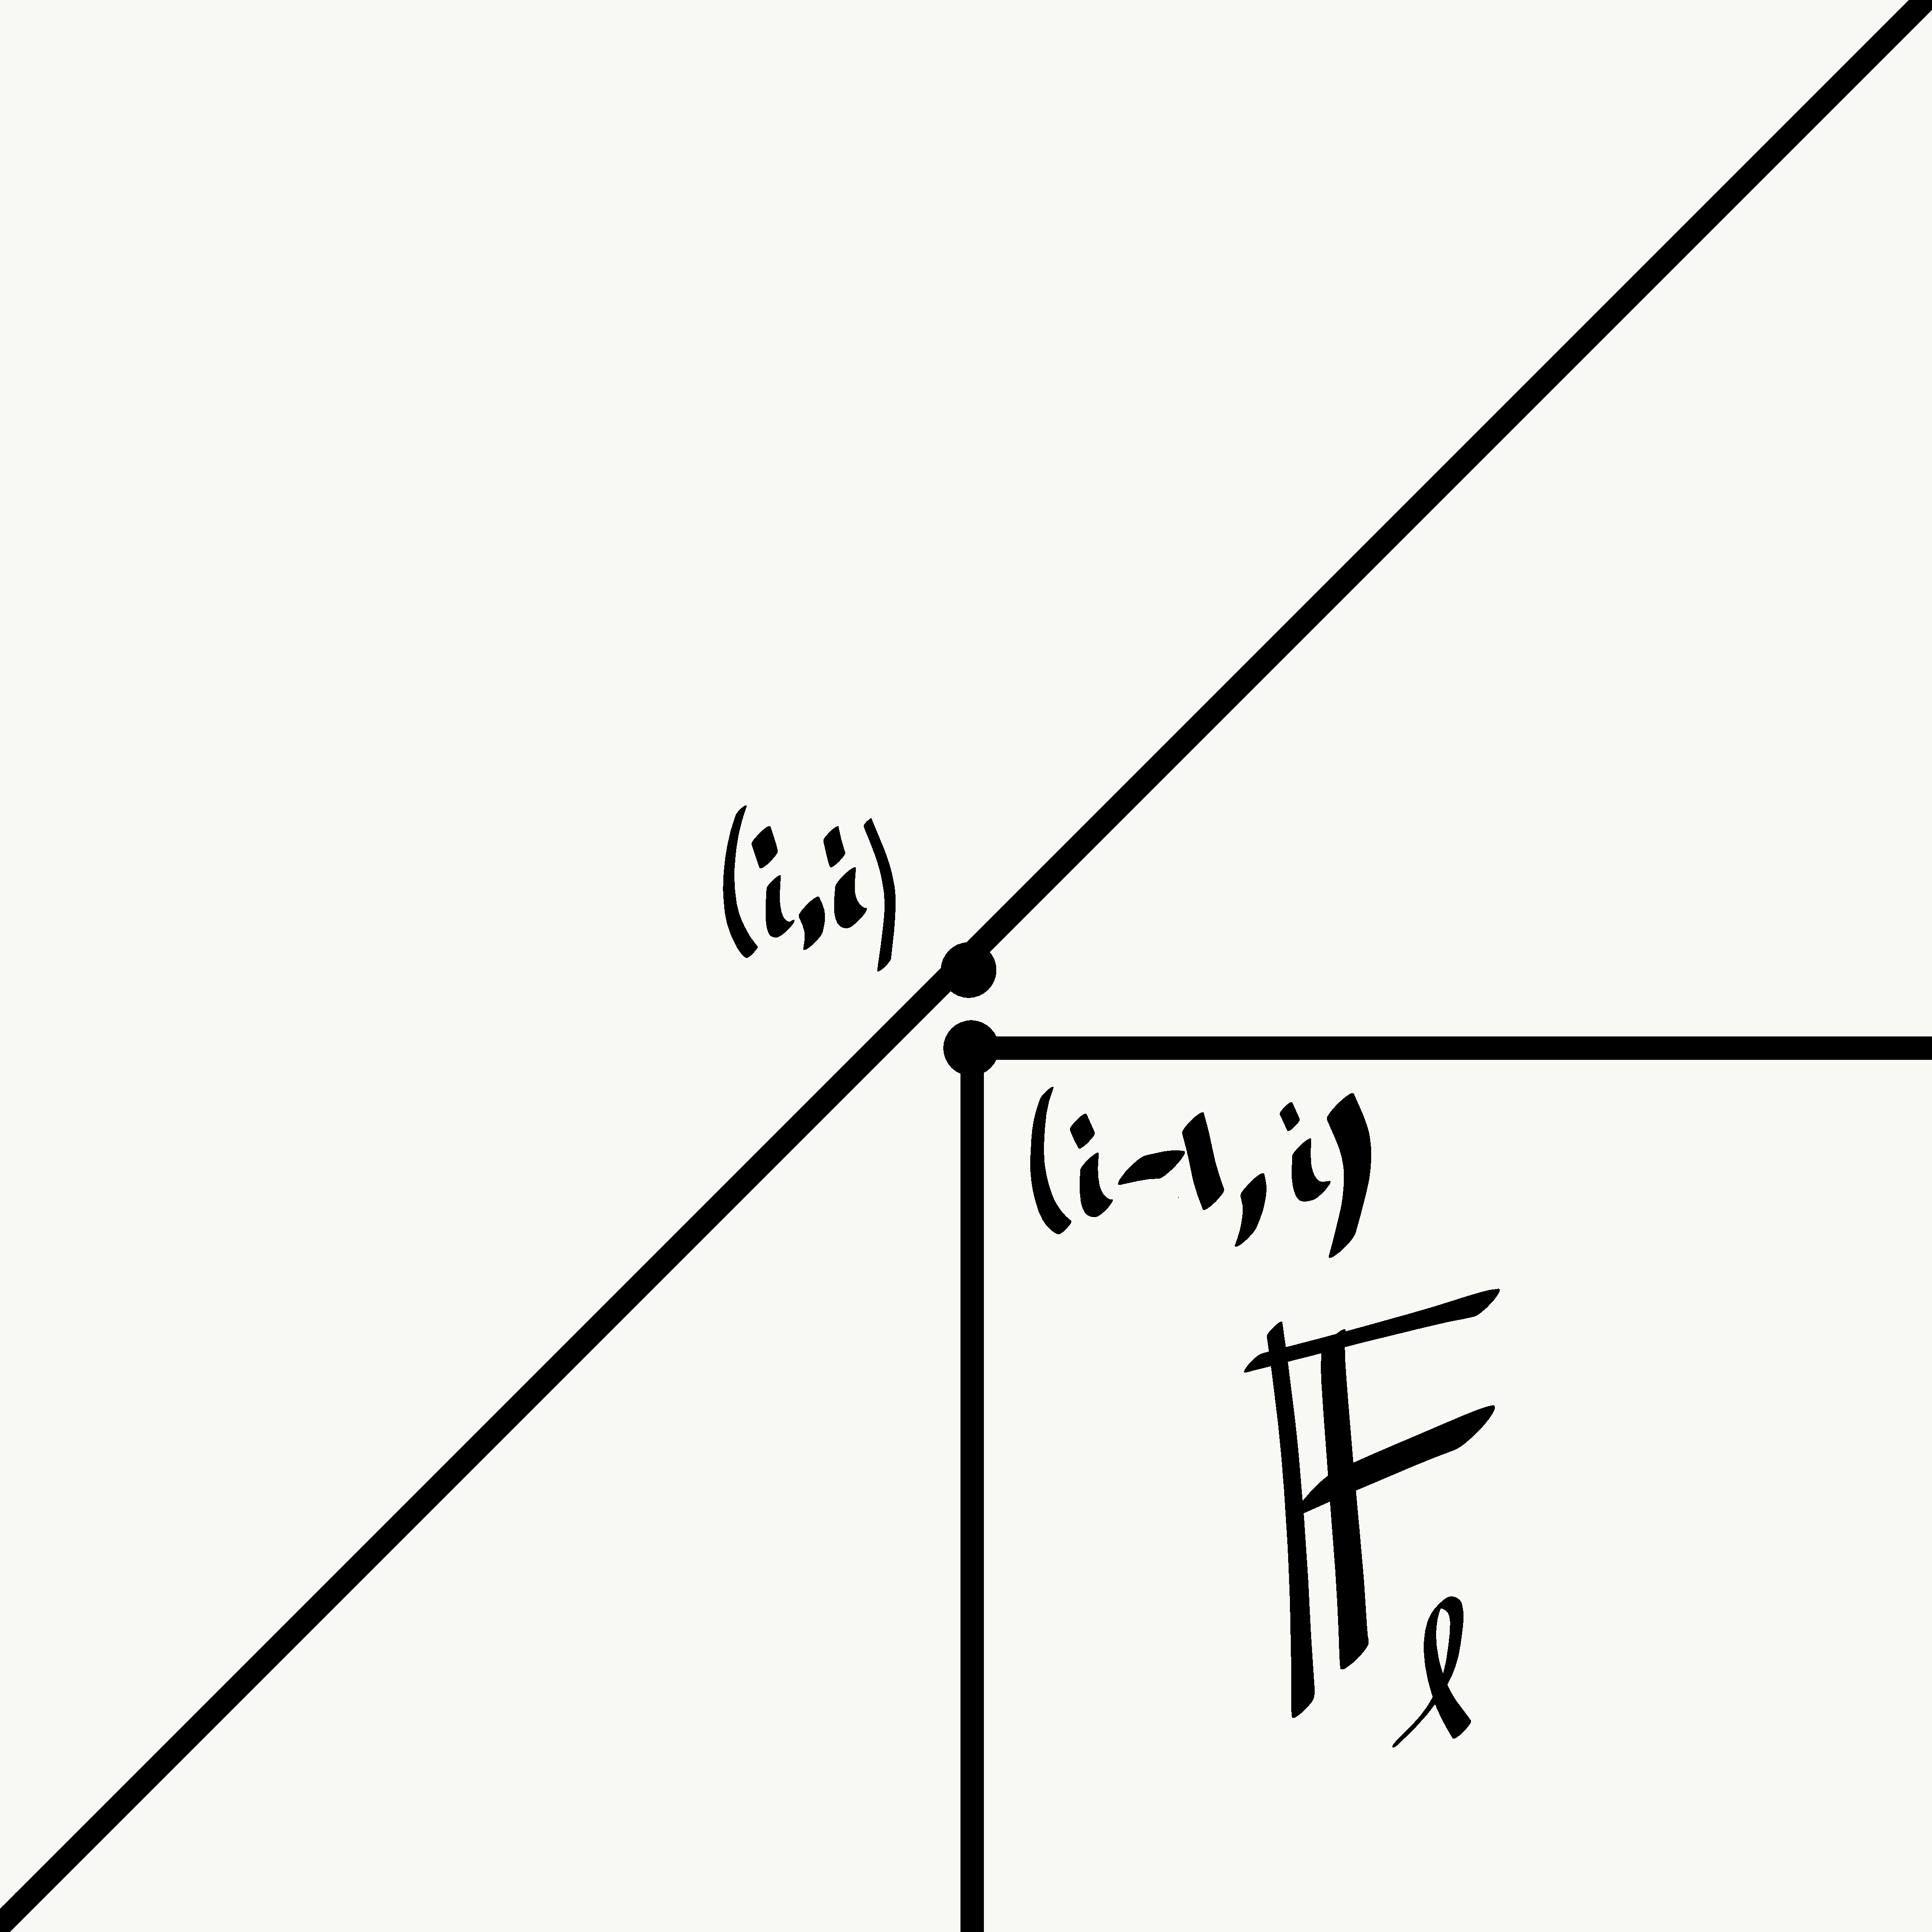
\includegraphics[width=.4\textwidth]{proind.pdf}\hspace{3em}
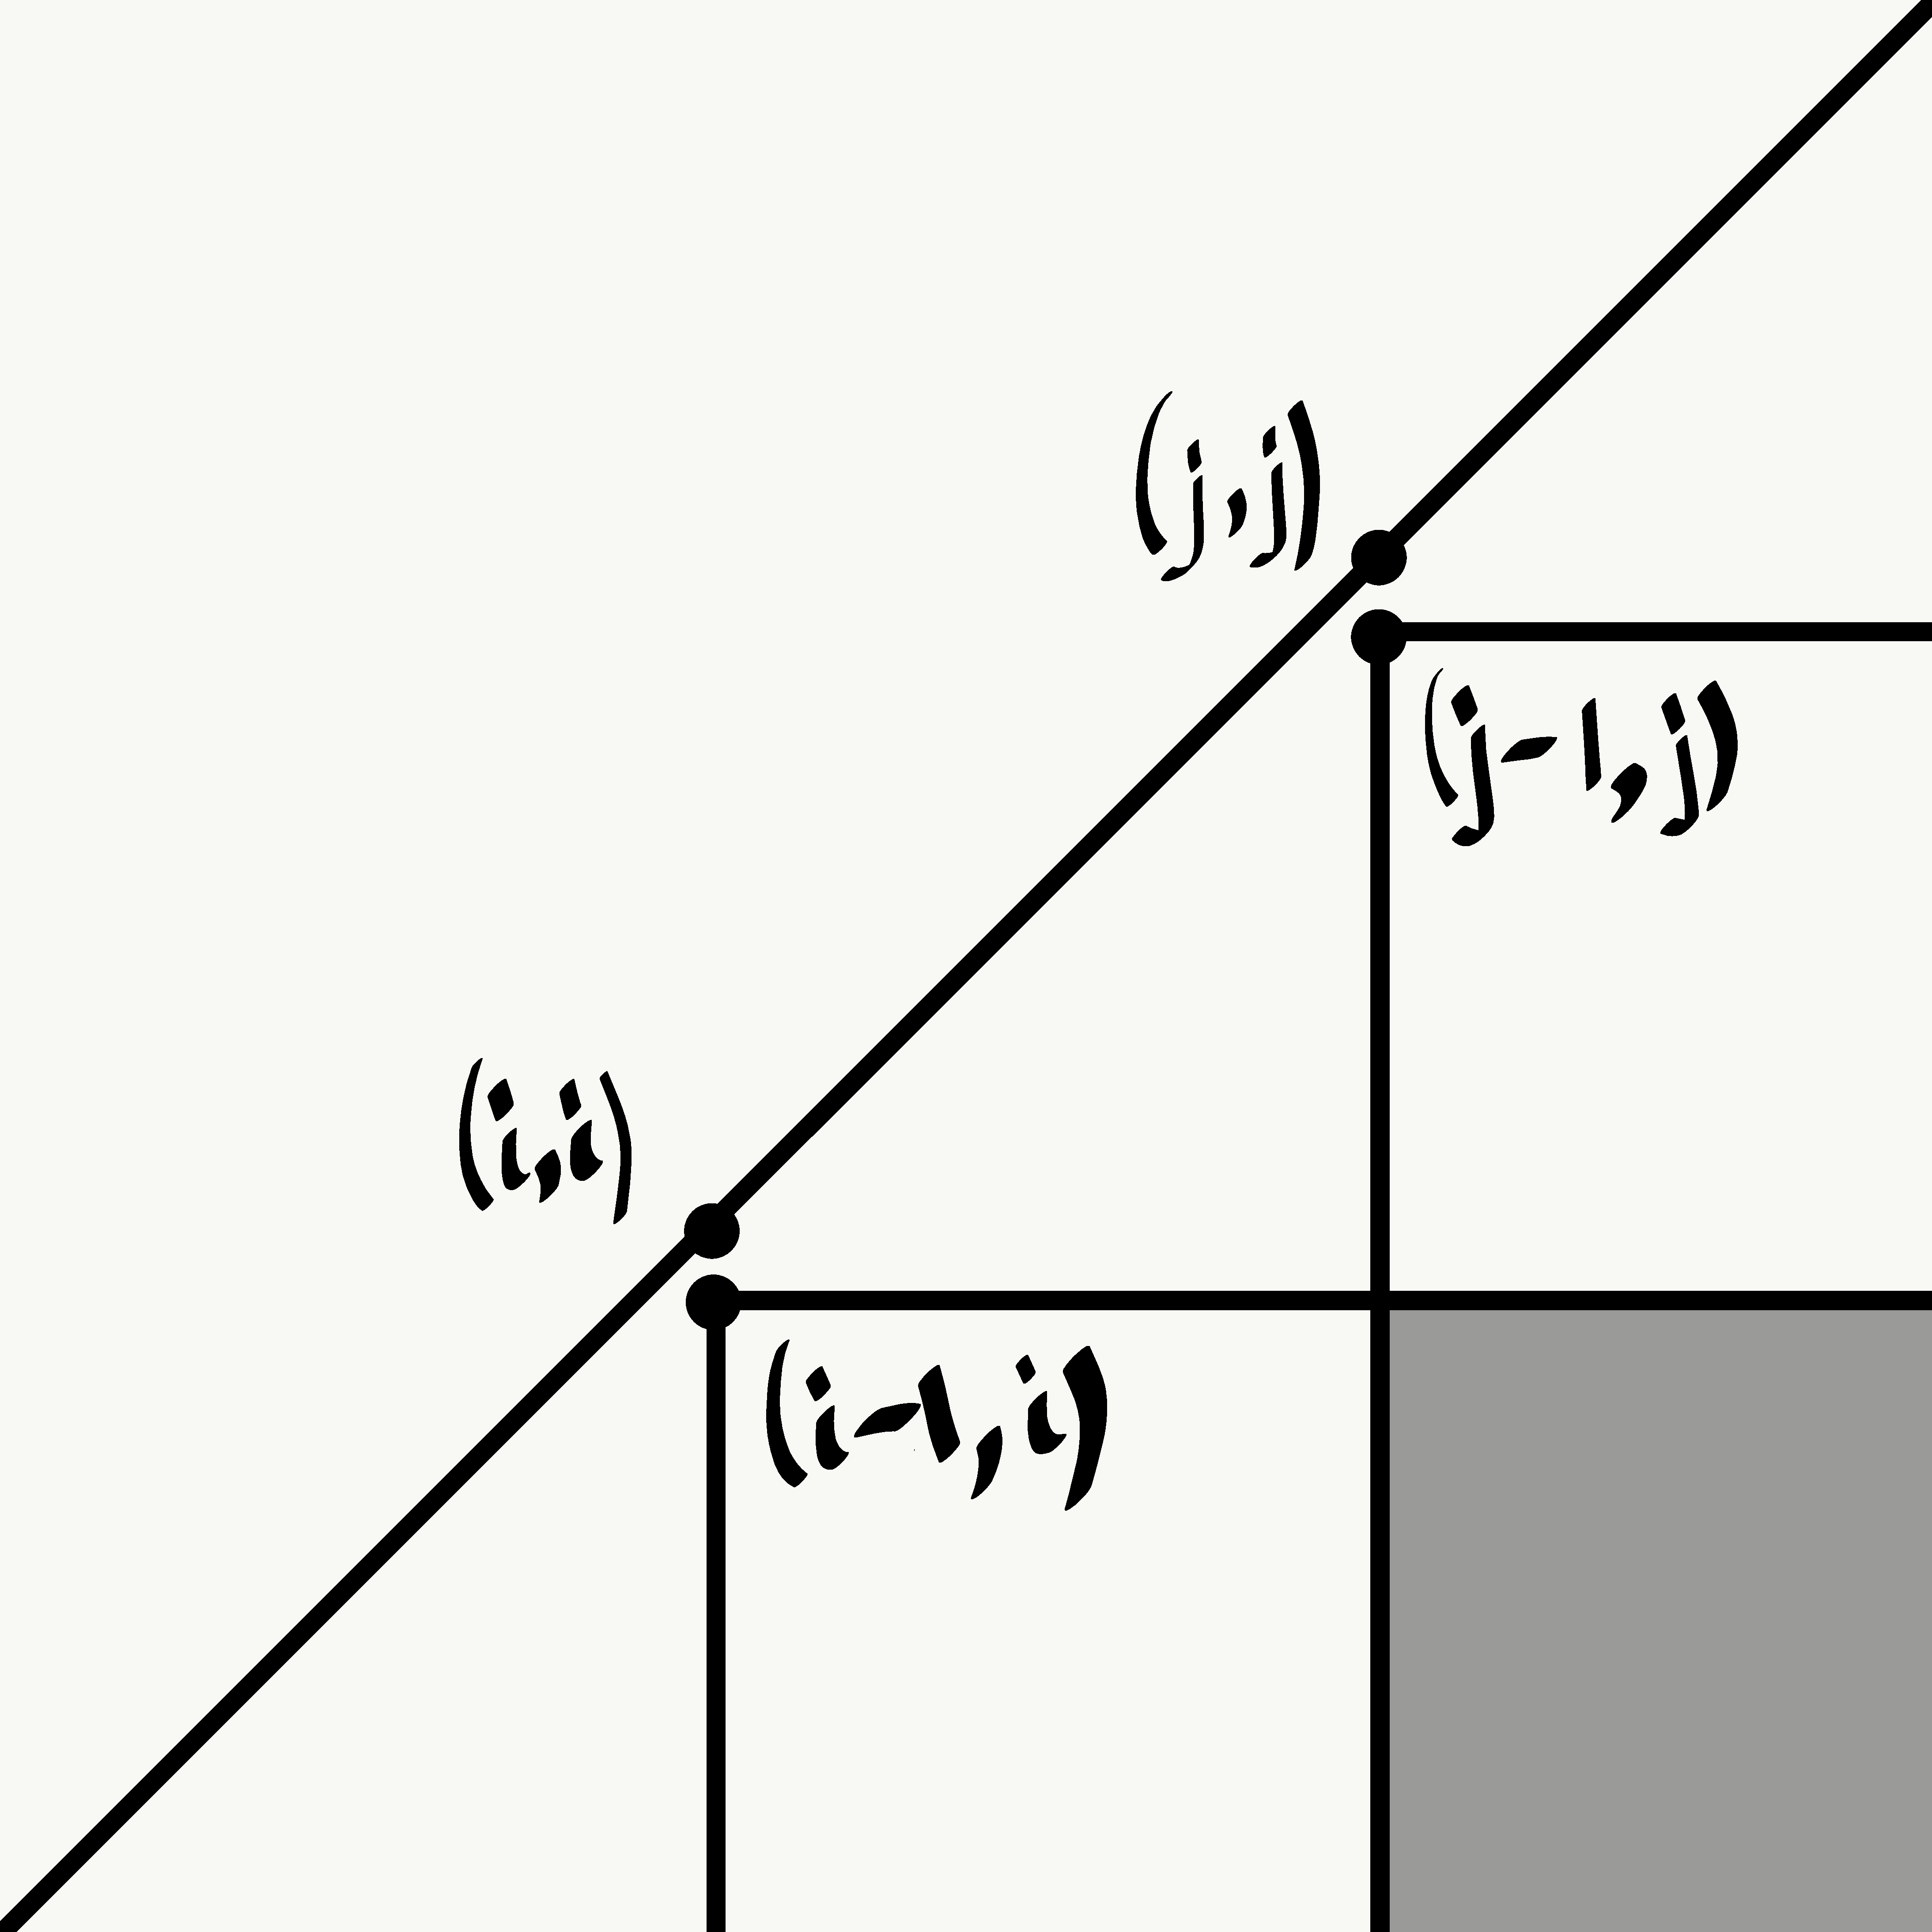
\includegraphics[width=.4\textwidth]{proind2.pdf}
\caption{}
\label{fig:proind}
\end{figure}
For, it is easily seen that
$\Hom_{\proind\mathcal P_{\overline k}}(\FF_\ell,\Aet)$
is in bijection with the data of a choice of $i\in\ZZ$ and a morphism in
$\Fil(\mathcal P_{\overline k})_a^\Pi$ from $\FF_\ell$, embedded as in the
left picture in Figure \ref{fig:proind}, to $\Aet$, modulo the
relation that two such morphisms are identified if they agree on their
nontrivial overlap, as indicated in the right picture in
Figure \ref{fig:proind}. If one associates to each nonzero Laurent series
$p\in A$ its initial form $\operatorname{in}(p)\in A^{a,a+1}$, there is a
unique morphism in $\Hom_{\proind\mathcal P_{\overline k}}(\FF_\ell,\Aet)$
with $\FF_\ell$ embedded as in Figure \ref{fig:proind} with $i=a$
corresponding to $p$. One recovers $A^a$ via the morphisms that can be
represented by a morphism in $\Fil(\mathcal P_{\overline k})_a^\Pi$ with
$\FF_\ell$ embedded in $i\leq-a$. Galois acts continuously on
$\Hom_{\proind\mathcal P_{\overline k}}(\FF_\ell,\Aet)=A$ for the 
topology induced by the filtration.

I do not see a way to make $\Aet$ into a ring, or a ring object.
The issue is of course that if we were dealing with an `étalization' of 
$A^\circ$, the multiplication would be easy to define as multiplication
respects the filtration. Once we pass to fractions, however, the
multiplication of two fractions no longer respects the topology.
As I understand it, $\Aet$ should be understood in analogy with the adic
formalism. The adic formalism, however, proceeds from the notion of $A$-
linear category, where $A$ is a commutative ring so that every object of the 
category has endomorphism ring an $A$-algebra. To define the category of
$\QQ_\ell$-sheaves, one formally inverts the endomorphism `multiplication by
$\ell$' in the $\ZZ_\ell$-category. In our case, the algebra $A$ (or, more
precisely, $A^\circ$) is not just a commutative ring, but a sheaf, a 
commutative ring with action of Galois. I have no doubt that $A^\circ$ can
be `étalized' in a very correct way, but it cannot be done directly from
the formalism of SGA 5 for this reason. The matter is essentially this:
the adic formalism in SGA 5 is enough to treat projective systems of étale
sheaves which are modules for a \emph{constant sheaf of rings} $\ZZ_\ell$,
which does not really enter the picture directly as a sheaf of rings, but
only via the commutative $A$ in the notion of $A$-linear category.
Of course, the notion of ringed topos is foundational, and so the way it is
done in the adic formalism is not really satisfactory. I wonder if the
pro-étale topos allows one to satisfactorily define an `$\ell$-adic sheaf of
rings' which needn't be constant. Our `étalization' of $A^\circ$ should be
such an `$\ell$-adic sheaf of rings.'

In the rest of the article, Sasha is trying to work `$\ell$-adically' for
an `nonconstant adic sheaf of rings' $A$. I think the $\proind$ formalism
isn't quite up to the job, because I do not see how to make $\Aet$ into a
ring object, and moreover I don't see how to have it act on $\Iet$. However,
I am not sure we actually need this. In the key lemma, forget the notion of
$\pi^{-1}$ and just notice that if $\ker$ and $\coker$ are annihilated by
a power of $\pi$ independent of $a,b$, say $N$, then both are killed by the
map $\id\ra\tilde\varphi_N$, which is an isomorphism in $\proind$.



\subsection*{1.4} Given $\pi\in A^{1*}$, let $\tilde t:=\exp\pi$ and 
$\gamma:=\tilde t-1$ so that $A\simeq\FF_\ell[[\gamma]]$ and
$\pi=\log\tilde t$.
(As remarked, if $t$ is a generator of the sheaf $\ZZ_\ell(1)$,
$\pi=\log t$ is a logical choice.)
The sheaf $I^{a,b}$ is defined by the action of the
group $G$ defined in \hyperref[glue:1.1]{the note to (1.1)},
and in view of the canonically split extension \eqref{glue:Gdef}, it will
suffice to show that if $l\in\ZZ_\ell(1),m\in\Gal(\overline k/k)$,
$lm\sigma_\pi(x)=\sigma_\pi(lmx)$.
Supposing $m=1$, the statement is clear as $l$ acts trivially on
$\ZZ_\ell(-n)$ (which is the reciprocal image of a sheaf on $\Spec k$)
and of course $\tilde l$ commutes with $\pi^n$ as both are elements of the
Iwasawa algebra $A$. In general, $m$ acts by multiplication by
$\chi(m)^{-n}$ on $\overline \pi^{-n}$ and sends
$\tilde t\mapsto\tilde t^{\chi(m)}$ so 
$m\pi=\log(\tilde t^{\chi(m)})=\chi(m)\pi$.


\addtocontents{toc}{\protect\setcounter{tocdepth}{-1}}
\begin{thebibliography}{BBD}
	\bibitem[B]{glue} \emph{How to glue perverse sheaves} par Beilinson
	\bibitem[BBD]{BBD} \textit{Faisceaux Pervers}
	par Beilinson, Bernstein, Deligne (\& Gabber!)
	\bibitem[Bühler]{buhler} Theo Bühler, \emph{Exact Categories}
\end{thebibliography}
\addtocontents{toc}{\protect\setcounter{tocdepth}{1}}
\end{document}
